\documentclass[a4paper,oneside,12pt]{article}

\usepackage[utf8]{inputenc}
\usepackage[T1]{fontenc}
\usepackage[french]{babel}
\usepackage{hyperref}
\usepackage{listings}
\usepackage{listingsutf8}
\usepackage{graphicx}


\newcommand{\airplug}{AIRPLUG}
\newcommand{\pie}{PIE}
\newcommand{\timestamp}{\textit{timestamp}}
\newcommand{\mdcinq}{MD5}
\newcommand{\hash}{\textit{hash}}

\newcommand{\chrisb}{Christophe Boudet}
\newcommand{\julien}{Julien Castaigne}
\newcommand{\chrisr}{Christophe Roquette}
\newcommand{\joe}{Jonathan Roudière}
\newcommand{\jeremy}{Jérémy Subtil}

\newcommand{\format}[1]{\begin{description}\item[Format] \texttt{#1}\end{description}}
\newcommand{\formatvar}[2]{\begin{description}\item[Format] \texttt{#1}~$\Rightarrow$ \texttt{#2}\end{description}}
\newcommand{\apgcmd}[1]{\texttt{#1}}
\newcommand{\fcmd}[2]{\texttt{#1\apgeq#2}}
\newcommand{\fkcmd}[1]{\texttt{#1}}
\newcommand{\fvcmd}[1]{\texttt{<#1>}}
\newcommand{\msgcmd}[1]{\texttt{#1}}



\title{Projet SR05 -- Réalisation d'une application répartie sur la plateforme \airplug}
\author{\chrisb, \julien, \chrisr,\\\joe, \jeremy}

\makeatletter
\hypersetup{
	colorlinks=true,
	linkcolor=blue,
	citecolor=blue,
	urlcolor=blue,
	pdftitle={\@title},
	pdfauthor={\chrisb, \julien, \chrisr, \joe, \jeremy},
	pdfsubject={\pie}
}
\makeatother

\lstdefinelanguage{algorithme}
{keywords={si,alors,finsi,sinon,pour,faire,finfaire,et,ou,non,envoyer,recevoir},
otherkeywords={<-},
comment=[l]//,
morecomment=[l][\bfseries\normalsize]**}
\lstset{language=algorithme,
frame=single,
numbers=left,
tabsize=2,
stepnumber=2,
extendedchars=true,
numberstyle=\tiny,
basicstyle=\small,
extendedchars=true,
inputencoding=utf8/latin1}


\begin{document}

\maketitle
\tableofcontents
\clearpage

%mainfile: rapport.tex

\section{Présentation du sujet}

\paragraph{}
Le choix de notre projet SR05 est de reproduire un réseau social tel que Twitter, de manière répartie, au travers de AirPlug.

\paragraph{}
Twitter est un réseau social permettant à ses membres de publier sur internet de courts messages (140 caractères). Les utilisateurs de Twitter peuvent s'abonner à d'autres membres du réseau social dans le but de pouvoir lire les messages rédigés par ces derniers.
Twitter est souvent utilisé par de grandes entreprises, des politiciens, afin de pouvoir être lus par plusieurs millions de personnes à travers le monde, mais aussi pour avoir un retour sur leurs actions. Il n'est pas rare de voir un service après-vente tel que celui de Dell, vous contacter si vous vous plaigniez d'un problème avec un de leurs produits sur Twitter.

\paragraph{}
Dans le cadre de SR05, nous allons faire de \pie, un réseau social proche de celui de Twitter avec cependant, quelques différences.
En effet, au lieu de fonctionner avec un système de serveurs centralisés au travers d'internet, nous allons utiliser un système réparti composé d'un ensemble de véhicules équipés d'AirPlug et de l'application \pie.
Un programme tel que \pie apporte un plus lors d'un trajet en voiture : non seulement nous pouvons suivre le flux de nos amis qui font route avec nous (convoi), mais aussi de tout autre inconnu. Ainsi, nous pouvons échanger un grand nombre d'informations avec les usagers nous entourants (dans la zone de diffusion). Grâce au système d'abonnement nous pouvons sélectionner les flux qui nous intéressent (collègues, informations routières, famille), tout en ignorant les autres (publicités, utilisateurs inintéressants\ldots).


%mainfile: rapport.tex

\section{Terminologie}

TODO julien/chrisB: définir les termes qu'on utilise pour décrire notre appli. Si c'est trop redondant avec la présentation, un zappe cette partie.

\begin{description}
	\item[abonnement]
	\item[message \pie]
	\item[voisins]
\end{description}


%mainfile: rapport.tex

\section{Algorithme réparti}

\lstinputlisting[caption={Algorithme réparti}]{algo.txt}

\subsection{Explication de l'algorithme}
\subsubsection{Initialisation}
Lors du démarrage de l'application, la base de donnée est reconstruite. Celle-ci comporte trois bases, plus une vue :
\begin{description}
	\item[bd\_abos] contient l'ensemble des identifiants de voitures, et pseudos d'utilisateurs auxquels nous sommes abonnés.
	\item[bd\_offres\_abo] contient l'ensemble des identifiants de voitures, ainsi que la distance des abonnements offerts à notre portée. Cette liste comporte des priorités, nous permettant de détruire les abonnements passagers dus à un simple croisement avec un véhicule.
	\item[bd\_demandes\_abo] a un fonctionnement identique à la base d'offres. Cependant, celui-ci intègre une partie des abonnements désirés par ces voisins.
	\item[bd\_flux] correspond à une vue des messages envoyés par nos abonnements.
\end{description}
\paragraph*{}
Un timer est ensuite enclenché afin d'effectuer à intervalle régulier un \texttt{HeartBeat}.

\subsubsection{HeartBeat}
Ce message correspond à un battement de c\oe ur, c'est à dire, une preuve d'existence. Il est diffusé à tous, mais ne pourra être relayé. Son contenu (offres et demandes du n\oe ud et de ses voisins environnants) servira à mettre à jour les bases de données des n\oe uds receveurs. Ce contenu pourra alors très bien figurer dans les messages \texttt{HeartBeat} des n\oe uds receveurs. Ce système permet de répartir la base de donnée générale des \textit{abonnements - abonnés} et ceci même lorsqu'aucun message \texttt{PIE} n'est transmis.

\paragraph*{}
Afin de former ce message, il faut tout d'abord nettoyer les bases de données. La priorité de chaque offre et demande va être décrémentée, afin que les n\oe uds que nous ne rencontrons plus aient une priorité négative. Cette priorité pourra être calculée, uniquement sur le nombre de messages \texttt{HeartBeat} de la cible, ou en prenant en compte les coordonnées GPS de celle-ci. Au contraire, à la réception d'un message, les abonnements contenus dans les offres et les demandes verront leur priorité incrémentée.

\subsubsection{Envoi et réception d'un message PIE}
Un message PIE correspond au message que l'utilisateur veut envoyer à ses suiveurs, de la même façon que sur \texttt{Tweeter}. Ce message doit donc être acheminé jusqu'à chaque voiture concernée par notre abonnement. Insérer une limite de distance dans la diffusion du message impliquerait un rayon de diffusion fixe, et ainsi, un long convoi de véhicules ne sera pas pris en compte. Augmenter la distance maximale de diffusion suppose une diffusion lointaine, probablement vers des zones n'ayant aucun intérêt pour notre abonnement. C'est pour cela que nous avons introduit deux notions : le TTL et le TTS.

\paragraph*{}
Le TTL (Time To Live) va être décrémenté chaque fois qu'une voiture retransmet le message alors que l'abonnement ne figure pas dans sa base de donnée \texttt{bd\_demandes\_abo}.
\paragraph*{}
Le TTS (Time To Survive) va être décrémenté par chaque voiture retransmettant le message alors que l'abonnement figure dans la base de donnée \texttt{bd\_demandes\_abo}.
\paragraph*{}
Un seul de ces deux compteurs peut être décrémenté. Le message n'est pas retransmis si le compteur devant être décrémenté est à 0. Ce mode de retransmission permet une diffusion intelligente. En effet, bien que le message puisse être diffusé inutilement dans un rayon égal au TTL, il pourra cependant s'étendre d'avantage dans les zones où un destinataire est présent, grâce au TTS. Le schéma ci-dessous montre ce principe.

\begin{center}
	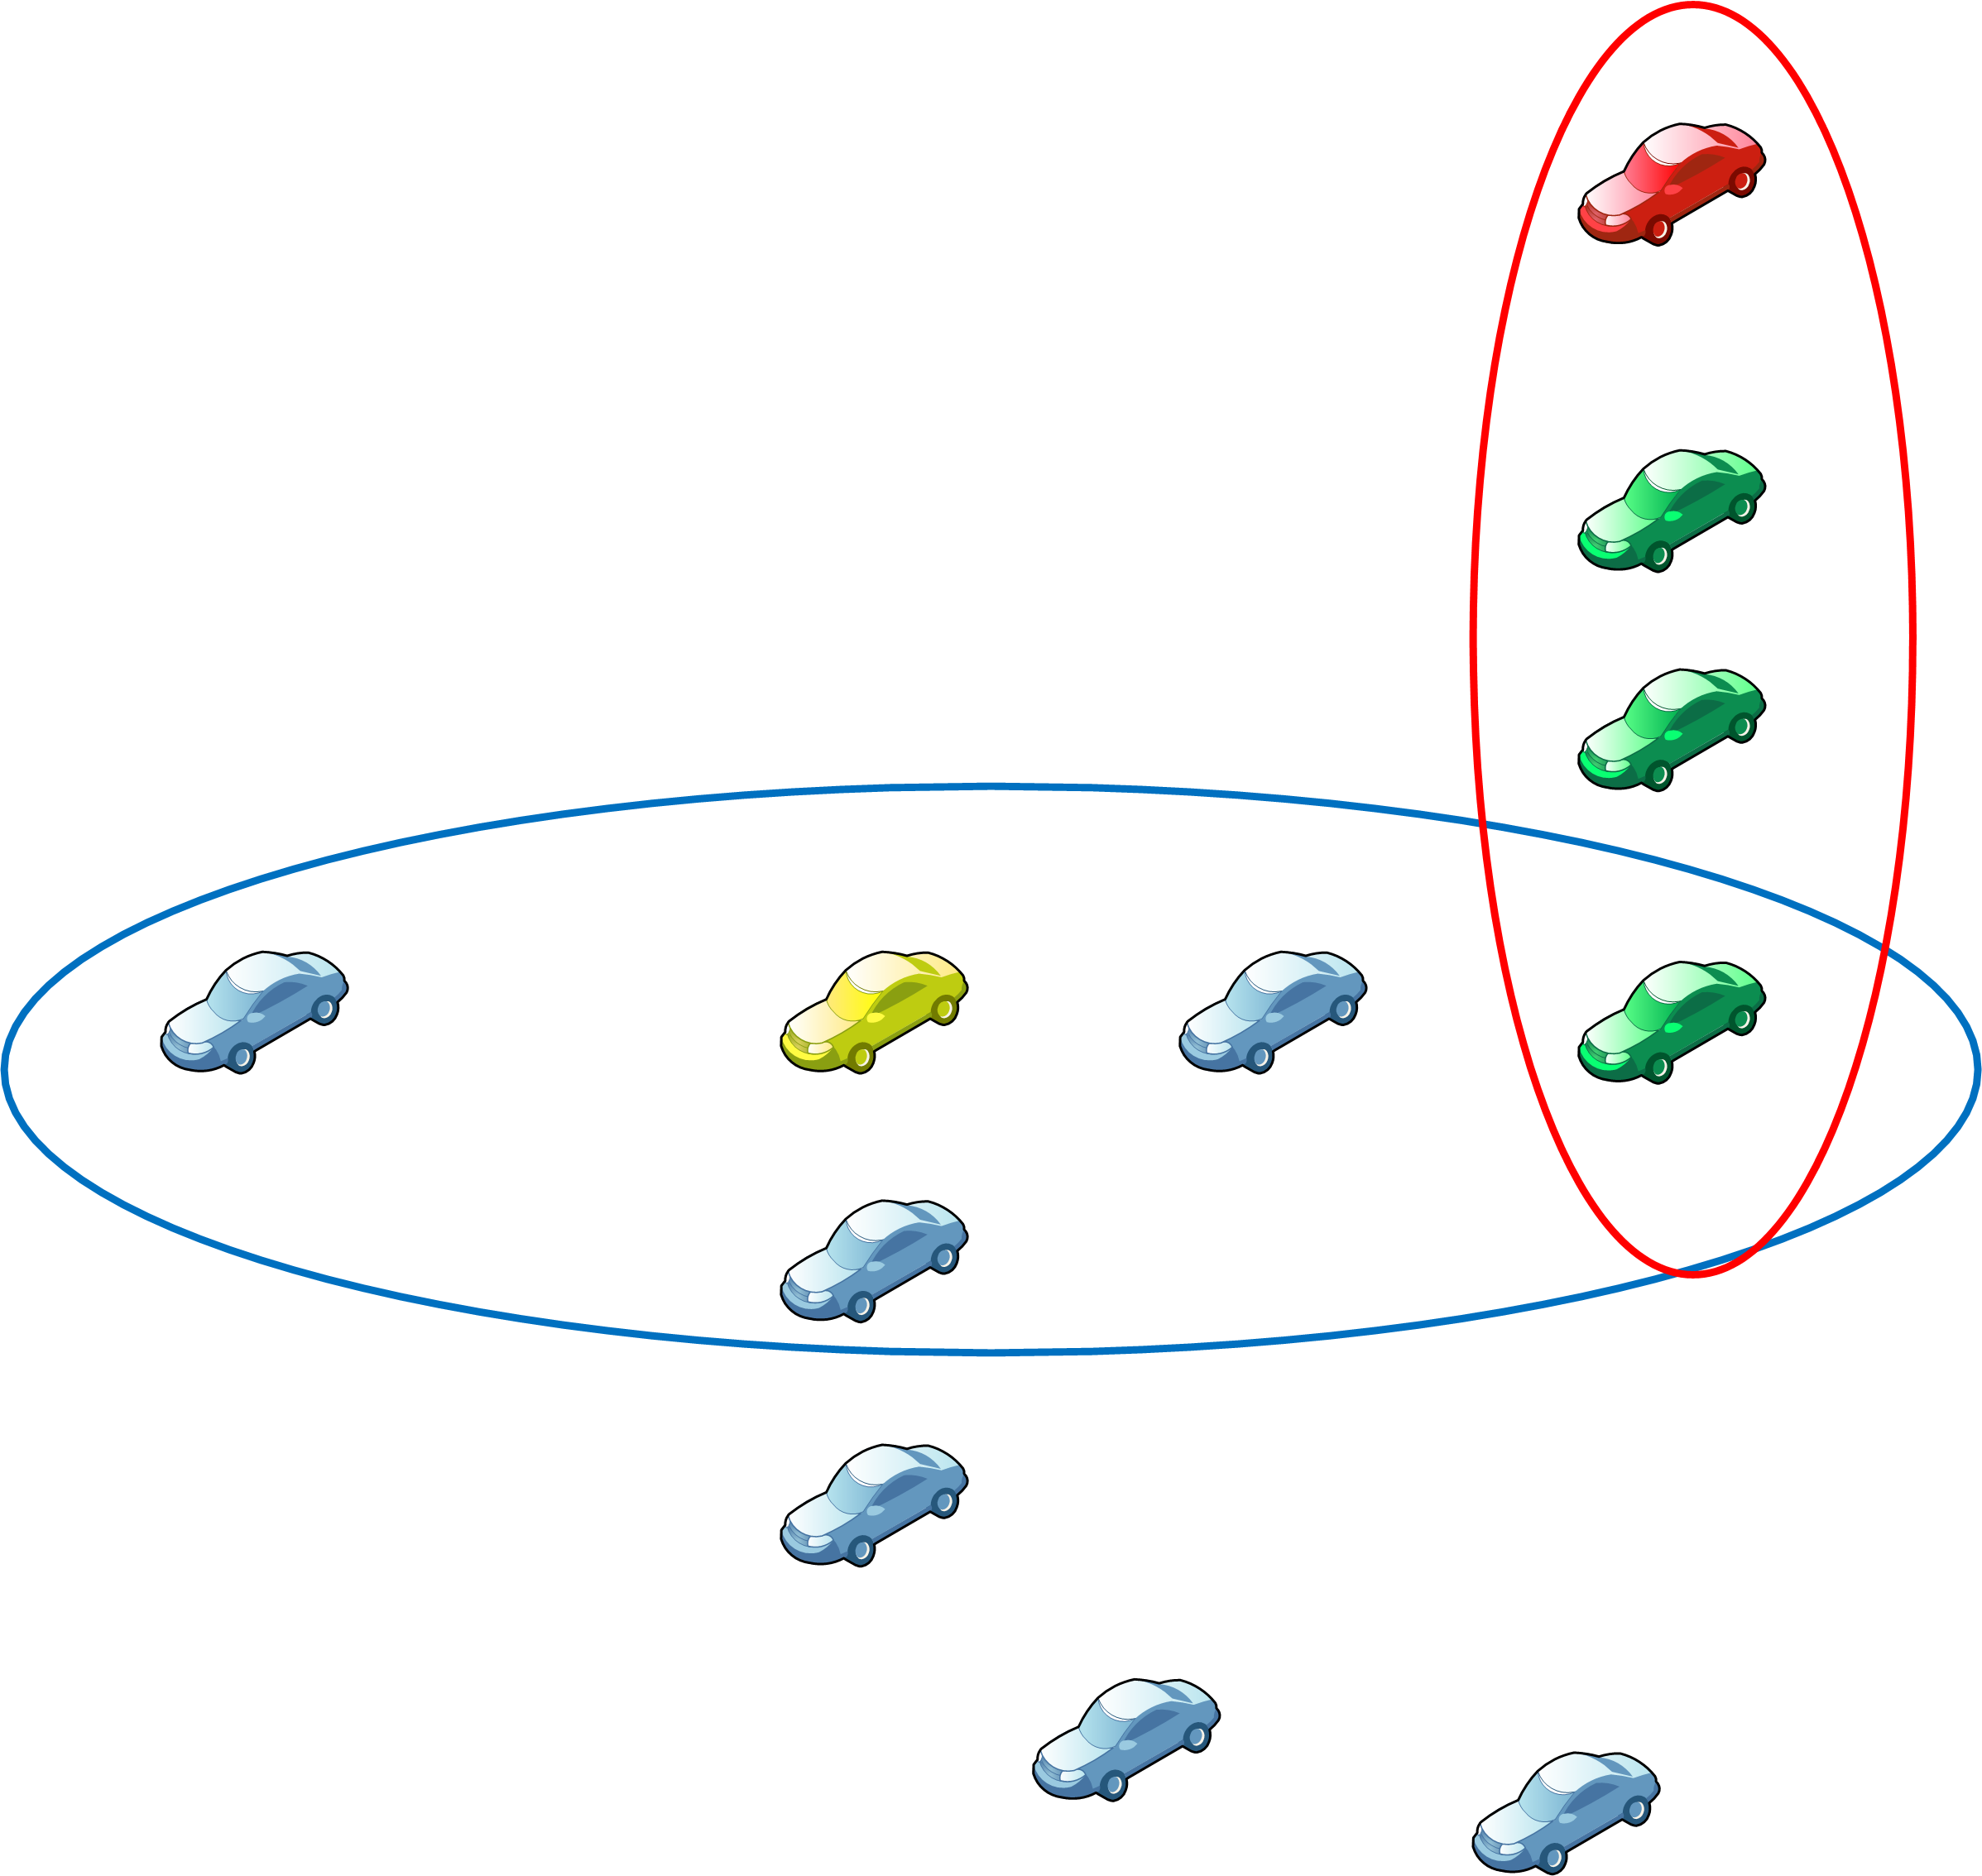
\includegraphics[width=0.75\textwidth]{img/schema2}
\end{center}

\paragraph*{}
\begin{description}
	\item[Voiture jaune :] N\oe ud émetteur du message PIE.
	\item[Voiture bleue :] N\oe ud non abonné et non intéressé par le message.
	\item[Voiture verte :] N\oe ud non abonné, mais connaissant un n\oe ud intéressé par celui-ci.
	\item[Voiture rouge :] N\oe ud abonné à l'émetteur désirant donc recevoir le message.
	\item[Ellipse bleu :] Zone de diffusion du message par décrémentation du TTL.
	\item[Ellipse rouge :] Zone de diffusion du message par décrémentation du TTS.
\end{description}
\paragraph*{}
Nous remarquons que contrairement à une diffusion par distance qui aurait un format de cercle, l'utilisation du TTL et TTS permet une diffusion ayant une forme variable. Dans le cas d'un convoi de véhicules, avec un véhicule égaré, cela va par exemple permettre de continuer à faire communiquer les deux protagonistes le plus longtemps possible.


\paragraph*{}
Dans un soucis d'optimiser chaque message, et d'avoir une convergence rapide entre les bases de données et la topologie physique de notre réseau de voitures, nous avons choisi d'inclure les offres et les demandes aux messages \texttt{PIE}. Ainsi ces messages participeront à un meilleur acheminement des futurs messages du réseau. Le réseau étant dynamique, les routes seront constamment réévaluées.

%mainfile: rapport.tex

\section{Protocole}

La définition du protocole de l'application \pie{} passe par la description des identifiants utilisés dans le système, ainsi que de celle du format des messages qui s'échangent dans le réseau.


\subsection{Identifiants}

Pour des raisons pratiques, un certain nombre d'objets de notre système doivent être identifiés.


\paragraph{Le n\oe ud}

Son identifiant est celui qui a été fourni à \airplug{} lors de son lancement.

\format{\fvnodeid}


\paragraph{La publication}

Son identifiant est défini par un \hash{}, calculé à partir de la date de sa rédaction et de l'identifiant du n\oe ud auteur.

\format{\fvmsgid}


\subsection{Formats de messages}
\label{section:mesg}

Les messages de l'application \pie{} sont composés :
\begin{enumerate}
	\item d'un entête ;
	\item d'un \payload, dont le format varie selon le type de message.
\end{enumerate}


\subsubsection{Entête}

Un entête commun a été défini pour tous les messages envoyés par l'application \pie.
Ses champs sont les suivants :

\begin{description}
	\item[\fkfrom] désigne l'émetteur d'origine du message. Ce champ n'est pas modifié en cas de relais du message par un n\oe ud voisin.
	\item[\fknick] désigne le pseudo de l'émetteur d'origine du message. Ce champ n'est pas non plus modifié en cas de relais.
	\item[\fkttl] correspond au nombre de sauts possibles parmi les n\oe uds n'ayant pas de voisin intéressé par le message.
	\item[\fktts] correspond au nombre de sauts possibles parmi les n\oe uds ayant un voisin intéressé par le message.
	\item[\fktype] indique le type du message, impliquant un certain format de \payload. Ce champ peut prendre les valeurs suivantes :
		\begin{itemize}
			\item \texttt{\msgheartbeat{} = 0}
			\item \texttt{\msgpie{} = 1}
		\end{itemize}
\end{description}

\format{\ffrom \apgdelim \fnick \apgdelim \fttl \apgdelim \ftts \apgdelim \\ \ftype \apgdelim \fvpayload}


\subsubsection{\Payload : message \msgheartbeat}

Le \heartbeat{} correspond à une annonce des offres et des demandes du n\oe ud lui-même ou de ses voisins, directs ou non.

Le \payload{} du message contient donc à la fois une liste d'offres et une liste de demandes.
Une entrée de ces listes comprend un identifiant de n\oe ud et une pondération associée.

Du fait de la taille limitée des messages \airplug, toutes les offres et demandes disponibles ne peuvent pas être annoncées via le message \msgheartbeat.
Ainsi, les entrées doivent être sélectionnées :

\begin{enumerate}
	\item les entrées correspondant aux n\oe ud sont choisies en priorité ;
	\item les entrées les plus importantes sont sélectionnées ;
	\item enfin, s'il reste de la place, on choisit aléatoirement des entrées pour compléter.
\end{enumerate}

Par ailleurs, les messages \msgheartbeat{} sont utilisés par un n\oe ud pour connaitre ses voisins.
En effet, il suffit de récolter le contenu des champs \fkfrom{} et \fknick{} de leurs entêtes.

\format{\foffers \apgdelim \fdemands}

\formatvar{\fvoffers}{\\\fvnodeid-\fvnick-\fvdistance,\fvnodeid-\fvnick-\fvdistance,\ldots}

\formatvar{\fvdemands}{\\\fvnodeid-\fvnick-\fvdistance,\fvnodeid-\fvnick-\fvdistance,\ldots}


\subsubsection{\Payload : message \msgpie}

Le message \msgpie{} correspond à l'envoi d'une publication d'un utilisateur.
Il contient alors les champs suivants :

\begin{description}
	\item[\fkmsgid] identifie la publication de façon unique. Il permet entre autres de savoir si un même message a été reçu plusieurs fois.
	\item[\fkmsgdate] correspond à la date de la rédaction de la publication.
	\item[\fkmsgcontent] correspond au contenu de la publication.
\end{description}

\format{\fmsgid \apgdelim \fmsgdate \apgdelim \fmsgcontent}


%mainfile: rapport.tex


\section{Structures de données}
\label{section:storage}

\subsection{Le modèle - vue d'ensemble}

Le modèle des structures de données utilisées par PIE est basé autour de la notion de
flux, à ce flux est associé un état. Ces flux sont caractérisés par un couple d'informations
garantissant leur unicité. Il s'agit de la provenance du flux - le champ FROM du protocole
(\cfsection{mesg}) - et de l'identité de l'utilisateur associé a ce flux - le champs NICK
du protocole (\cfsection{mesg}).\\

En plus de celles précitées, un flux est un objet constitué d'un ensemble de caractéristiques.
Ces caractéristiques sont d'une part les informations liées à la notion d'identité de utilisateur
associé au flux, de l'autre celles liées - au même titre que l'état - à sa gestion. \\

Les informations caractérisant un utilisateur associé à un flux ne sont pas - par défaut -
transmises par celui-ci (à l'exception du couple NICK/FROM). Lorsque 
l'utilisateur local de PIE en fait la demande, une requête unidirectionnelle (de type \textbf{getinfo})
peut alors être adressée au flux en question; si une réponse de sa part est reçu alors
les informations le concernant sont mises à jour. \\

Du fait de leur unicité, les flux constituent un ensemble, une collection d'objets uniques (\cfsection{vin}).
L'état définit une relation entre un flux et l'utilisateur local de l'application. Un flux
peut être : \\

\begin{itemize}
	\item \textbf{available}, l'utilisateur local a accès à ce flux,
    \item \textbf{forwarded}, l'utilisateur local transmet le flux à des paires,
    \item \textbf{subscribed}, l'utilisateur local est abonné au flux. \\
\end{itemize}

Ces états possibles se superposent, car un flux peut avoir les trois états simultanément.
L'état d'un flux est une caractéristique offrant les relations ensemblistes suivantes : \\

\begin{itemize}
	\item quelque soit un flux x alors il appartient à \textbf{available},
	\item \textbf{subscribed} est un sous ensemble d'\textbf{available},
	\item \textbf{forwarded} est un sous ensemble d'\textbf{available},
	\item \textbf{subscribed} U \textbf{forwarded} est inclus ou égale à \textbf{available},
	\item L'intersection de \textbf{subscribed} et \textbf{forwarded} est éventuellement non vide.\\
\end{itemize}

L'état d'un flux est une caractéristique de gestion, cette caractéristique est modélisée
par l'utilisation de trois listes : \\

\begin{itemize}
	\item la liste des flux \textbf{available}, soit l'ensemble des flux,
	\item la liste des flux \textbf{forwarded}, le sous-ensemble des flux transmis,
	\item la liste des flux \textbf{subscribed}, le sous-ensemble des flux auquel l'utilisateur local est abonné. \\
\end{itemize}

Un gestion unifiée de ces structures de données est offerte par un sous-système de PIE,
l'interface de stockage. Cette interface permet la manipulation des flux, des informations 
qui leur sont associées et de leurs états, c'est l'interface de plus haut niveau pour la
manipulation des flux. L'interface de stockage est une interface de gestion, automatisant
les différentes taches inhérentes à cette gestion, elle met à profit les relations ensemblistes 
exposées à travers l'utilisation de listes. \\

Le schéma suivant présente les structures de données précitées et les relations (logiques)
entre chacunes :  \\

\begin{center}
    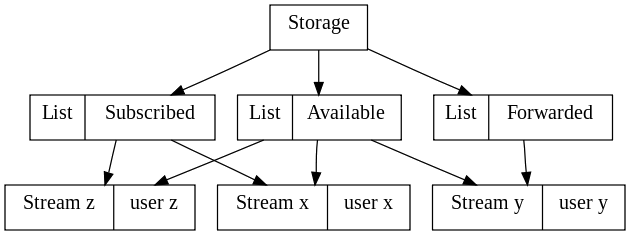
\includegraphics[width=0.8\textwidth]{img/struct.png}
\end{center}

\subsection{Implémentation}

Le modèle présenté dans le précèdent paragraphe a conduit à l'implémentation
présentée maintenant. Chacun des objets considérés dans le modèle dispose d'une
interface qui lui est propre. Il y a donc quatre interfaces de gestion différentes : \\

\begin{itemize}
	\item \textbf{user} : interface de gestion des utilisateurs associés aux flux,
	\item \textbf{stream} : interface de gestion des flux,
	\item \textbf{list}:  interface de gestion des listes de flux,
	\item \textbf{storage} : l'interface de stockage, plus haut niveau d'abstraction. \\
\end{itemize}


Chacune des interfaces précitées offre une couche d'abstraction permettant la manipulation
des objets qu'elle modélise. Elles sont définies par deux niveaux : Il y a d'une part, des
fonctions de manipulation globales des objets fournis par l'interface (telle que seraient
des fonctions statiques d'une classe en java) et de l'autre ,des fonctions de manipulation
des objets par eux mêmes (le pendant des méthodes en java). Les fonctions et méthodes des
différentes interfaces permettent par exemple la recherche d'objets en fonction de la valeur
de leur attributs autant que leur mise à jour ou encore leur destruction.

\subsubsection{Interface User}

Un utilisateur (\textbf{user}) est représenté par un objet disposant
d'un certain nombre de caractéristiques, celles ci sont : \\

\begin{itemize}
	\item \textbf{id} : information de gestion initialisée à la création,
	\item \textbf{nickname}	: correspond au champ \textbf{NICK} définit dans le protocol,
	\item \textbf{email} : l'adresse email de l'utilisateur (optionnelle),
	\item \textbf{fullname} : son nom (optionnelle),
	\item \textbf{firstname} : son prénom (optionnelle),
	\item \textbf{phone\_nb} : son numéro de téléphone (optionnelle),
	\item \textbf{age} : son age (optionnelle),
	\item \textbf{sex} : son sexe (optionnelle),
	\item \textbf{dest} : sa destination actuelle (optionnelle),
	\item \textbf{desc} : se description de l'utilisateur (optionnelle).\\
\end{itemize}

Les caractéristiques notées optionnelles sont celles n'ayant pas d'impact
sur le fonctionnement de PIE en interne, elles n'ont pour objet que d'offrir
un profil plus détaillé (informations obtenues par une requête \textbf{getinfo}).
 
\subsubsection{Interface Stream}

Ces objets utilisateur, sont implémentés en utilisant le package Itcl qui offre
une couche abstraction de type objet au langage TCL, ils sont contenus
(associés) dans un object de type flux (\textbf{stream}). L'objet \textbf{stream}
est defini par les champs : \\

\begin{itemize}
	\item \textbf{stream\_id} : information de gestion initialisée à la création,
	\item \textbf{car\_id} : information correspondant au champ FROM du protocol,
	\item \textbf{time\_available} : l'heure locale depuis laquelle le flux est disponible,
	\item \textbf{time\_lastmsg} : l'heure locale du dernier message reçu de ce flux,
	\item \textbf{time\_lasthello} : l'heure locale du dernier message de type hello,
	\item \textbf{nb\_mesg} : le nombre de messages envoyés par ce flux,
	\item \textbf{user} : l'objet utilisateur présenté dans le précédent paragraphe,
	\item un certain nombre d'informations de gestion pour le protocole.
\end{itemize}

\subsubsection{Interface List}

Les listes bien que nativement présentent dans le langage TCL bénéficient également
d'une interface particulière et écrite par nos soins. Cette interface permet une gestion
cohérente au modèle ensembliste - unicité des éléments dans chaque liste.

\subsubsection{Interface Storage}

Enfin l'interface de stockage est celle permettant la gestion de l'ensemble, c'est 
celle présentant le plus haut niveau d'abstraction, c'est donc à travers cette interface
que sont manipulés tous les objets du modèle. Le stockage maintient 4 listes :\\

\begin{itemize}
	\item la liste des flux \textbf{available}, soit l'ensemble des flux,
	\item la liste des flux \textbf{forwarded}, sous-ensemble des flux transmis,
	\item la liste des flux \textbf{subscribed}, sous-ensemble des flux souscrits localement,
	\item la liste des flux \textbf{forgotten}, les flux devenus indisponible. \\
\end{itemize}

Lorsque un nouveau flux est crée, cela correspond à la réception d'informations de sa part, l'objet
associé à ce flux est alors initialisé. Il est crée à travers l'interface de stockage des flux et
bénéficie de l'état disponible (\textbf{available}). Si l'utilisateur décide de s'y abonner, alors
le flux bénéficie également de cet état et à ce titre, est mis dans la liste associée (\textbf{subscribed}).
Enfin un flux pour lequel PIE est informé qu'il intéresse un pair, sera mis dans la liste des flux
transmis (\textbf{forwarded}). \\

Lorsqu'un flux devient indisponible, plutôt que de détruire l'objet associé, celui-ci est placé dans la
liste \textbf{forgotten}, il tombe dans les limbes. Il s'agit d'une optimisation et d'un écart au modèle
présenté : ne pas détruire ce flux permet de le rendre disponible de nouveau à l'utilisateur local et
cela sans sur-coup au niveau des ressources locales. De plus, si d'aventure, des informations avaient
au préalable été obtenues sur l'utilisateur associé au dit flux (via une requête de type getinfo) alors
il n'est pas nécessaire de les redemander ensuite, ce qui évite de saturer le média de communication. \\

L'évolution des états d'un flux peut être repésenté par le schéma suivant :

\begin{center}
    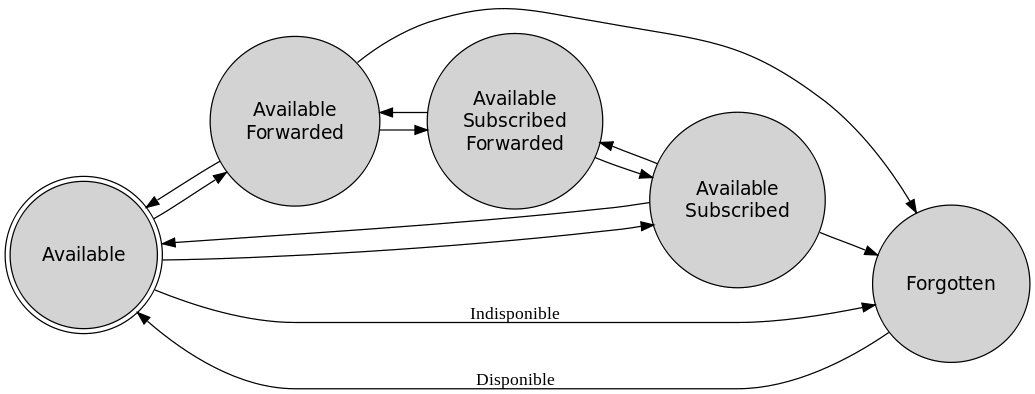
\includegraphics[width=1\textwidth]{img/state.png}
\end{center}

Les listes ne contiennent en fait que des références vers les objets. C'est à l'interface de
stockage de garantir les propriétés précédemment exposées. \\


%mainfile: rapport.tex

\section{Interface graphique (IHM)}
\label{section:ihm}

\subsection{Présentation}

L'interface graphique permet l'utilisation de PIE par l'utilisateur local. Elle a pour vocation
de présenter une vue la plus complète possible de l'état de l'application à l'utilisateur. Ceci
est réalisé à travers neuf onglets et une fenêtre. Un menu permet de changer l'état de l'application
et les vues (onglets/fenêtre) proposées. \\

\textbf{PIE's interface} : l'onglet principal. Il offre une vue à l'utilisateur des flux disponibles,
des flux auxquels l'utilisateur est abonné et une zone de texte afin que ce dernier puisse écrire et
envoyer des messages (voir capture ci-dessous). Cet onglet est tout le temps ouvert. Il est possible
de s'abonner ou se désabonner d'un flux en le faisant glisser de la zone référençant les flux disponibles
vers celles référençant les flux auxquels l'utilisateur est abonné et vice-versa (drag and drop).\\

\begin{center}
    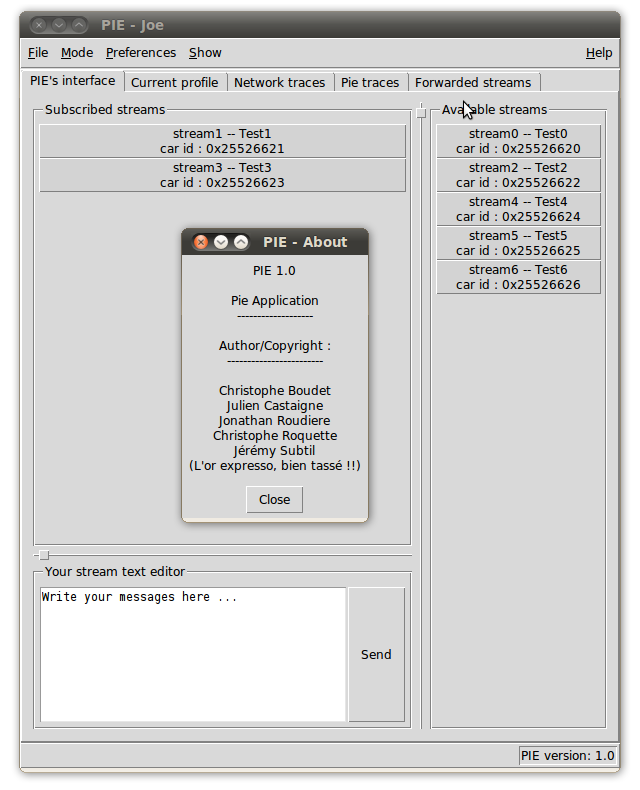
\includegraphics[width=0.9\textwidth]{img/pie-main.png}
\end{center}

\clearpage
\textbf{Current Profile} : onglet permettant la consultation et la modification du profil
courant de l'utilisateur local. Si le profil est modifié, il est alors enregistré. \\

\begin{center}
    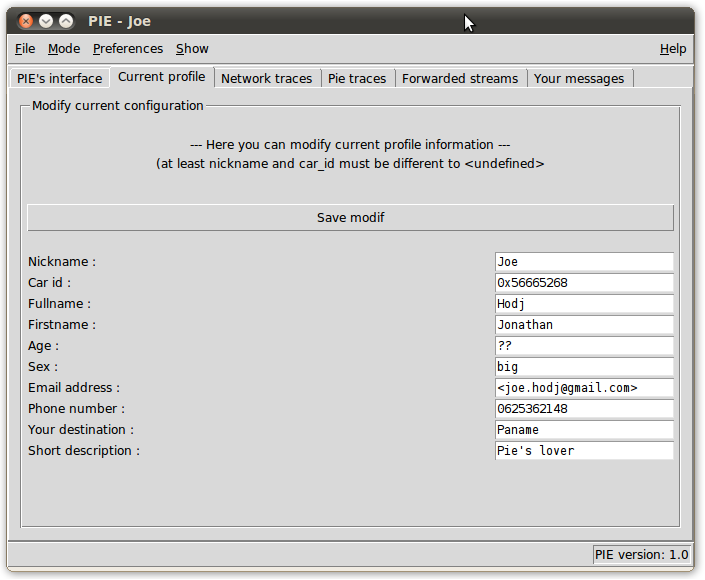
\includegraphics[width=0.9\textwidth]{img/profile.png}
\end{center}

\textbf{Global settings} : onglet permettant la consultation et la modification des réglages 
d'ordre général de PIE (les onglets ouverts au démarage de l'application ou le mode par défaut). \\

\textbf{Your messages} : onglet qui permet de consulter les précédents messages envoyés par l'utilisateur local. \\

\textbf{Forwarded streams} : onglet qui permet de consulter les flux qui sont transmis à des pairs, de mettre à jour 
les informations affichées et éventuellement d'arrêter la transmission de ce flux.\\

\begin{center}
    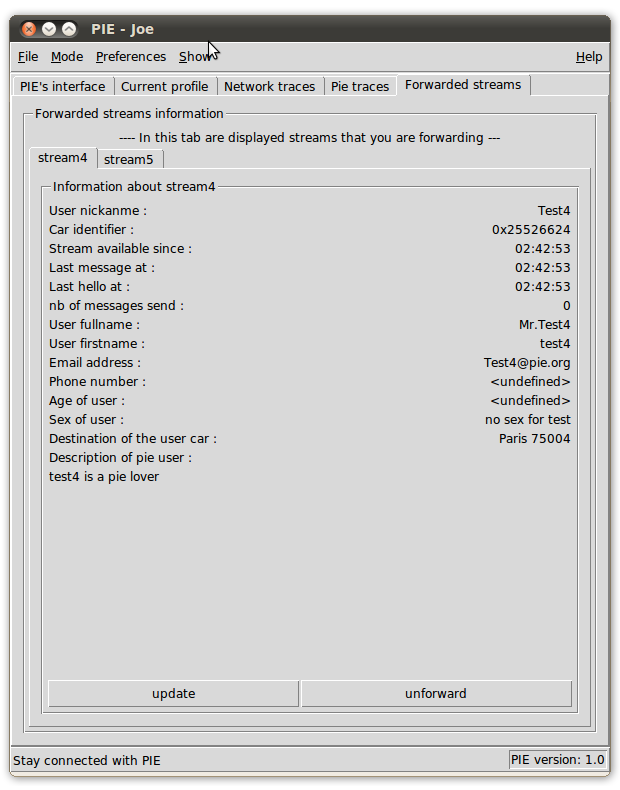
\includegraphics[width=0.9\textwidth]{img/forwarded.png}
\end{center}

\textbf{Subscribed streams} : fenêtre permettant de voir les flux auxquels l'utilisateur local est abonné, chaque flux est affiché dans un onglet.
Les informations concernant le flux sont affichées ainsi que les messages qu'il a émis.\\

\begin{center}
    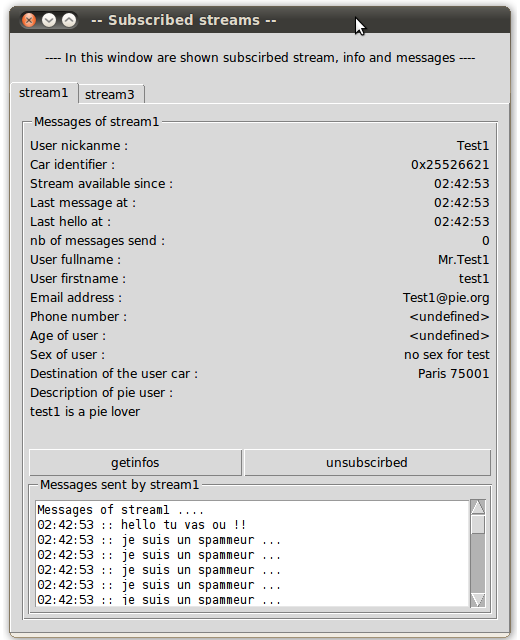
\includegraphics[width=0.9\textwidth]{img/subscribed.png}
\end{center}

\textbf{Pie traces} : onglet qui affiche toutes les traces (debug) de l'application et de ses sous-systèmes.\\

\textbf{Network traces} : onglet qui permet de consulter l'ensemble des messages émis ou reçus depuis le réseau dans leur forme brute.\\

\textbf{Input/Output traces} : deux onglets qui permettent de consulter l'ensemble des messages reçus/émis depuis le réseau dans leur forme brute. \\

\section{Comptes utilisateurs et configuration}

PIE utilise deux fichiers de configuration, le premier est celui définissant le profil de l'utilisateur
alors que le second permet de configurer l'application elle même (onglet ouvert, mode, ...).  \\

Les fichiers de configuration sont conservés dans le répertoire \textbf{\$HOME/.pie} (par défaut), le fichier
de configuration globale doit s'appeler \textbf{global.conf} et les fichiers de profil utilisateur doivent
s'appeler \textbf{NICKNAME.conf}. \\

A son lancement l'interface graphique vérifie à travers le sous-système de gestion des configurations
que le répertoire de configuration et les fichiers précités sont présents. Si ce n'est pas le cas, alors le
répertoire de configuration et un fichier de configuration globale générique sont crées. L'utilisateur, lui,
est invité à définir un profil via l'IHM. \\

Si plusieurs profils utilisateur sont disponibles alors l'utilisateur est invité à en choisir un. Une fois ces
vérifications faites et un profil déterminé l'application PIE est prête à être utilisée.


\section{Fonctionnalités}


%mainfile: rapport.tex
\section{Évolutions possibles}
Dans cette version de \pie, nous nous sommes concentrés sur l'implémentation de notre algorithme et donc sur la spécificité du routage.
Afin de permettre une évolution de l'application, nous avons tenté de respecter au maximum la philosophie \airplug{} dans le nommage des variables et procédures.
D'autre part, chaque fonction est documentée et chaque structure a été pensée modulable afin de ne pas limiter les possibilités de \pie{} à sa version actuelle. 

\subsection{Gestion des utilisateurs}
\airplug{} donne la possibilité aux utilisateurs d'une voiture de communiquer grâce à des application via la borne wifi. Mais que se passe-t-il si plusieurs personnes dans la voiture décide d'utiliser \airplug{} ?
Dans un tel cas, l'identité de la voiture ne suffit plus, mais il faut identifier chaque personne de la voiture. Pour ce faire, nous avons mis en place la structure d'utilisateurs évoquée précédemment. Dans le contexte de \pie, nous pouvons envisager rapidement de permettre à un utilisateur de récupérer les informations des propriétaires des flux qu'il suit. Ceci pourra être réalisé simplement par l'utilisation de deux nouveaux types de messages : un type pour effectuer la demande d'information, et un autre pour la réponse. Dans le cas d'une demande, nous pouvons imaginer qu'étant donné que chaque n\oe ud peut posséder l'information, il ne sera pas nécessaire que la réponse provienne du propriétaire du flux, mais de toute personne possédant ces données. 

\subsection{Connaissance des followers}
Dans la version actuelle de \pie, il n'est pas possible pour un utilisateur de connaitre l'identité des personnes intéressées par son flux. 
Cependant, cela pourrait être envisagé en ajoutant un type de message spécial demandant à chaque \etranger{follower} de décliner son identité au propriétaire du flux. 
Il est par ailleurs possible de réaliser une première liste grâce au partage des demandes entre les n\oe uds. Ainsi un ajoutant une information sur la personne qui demande, nous pourrions croiser nos données en regardant dans notre liste forwarded, les n\oe uds qui désirent notre flux. Cette liste ne serait pas complète étant donné que nous n'avons pas forcément reçu la demande de tous les n\oe uds, même éloignés. 

\subsection{Des applications tierces}
En ajoutant la gestion des identités, nous pouvons imaginer des applications tierces, utilisant \pie{} comme couche pour l'envoi de messages. Ces applications pourraient entre autre utiliser les destinations des utilisateurs pour proposer divers services comme du guidage, des points de rencontre dans le cas de longs trajets.


\end{document}

